\newpage 

\subsection{Building Transistors: The Chemistry of Silicon}

\noindent
To even begin to manage currents and voltages, we will need a way to control the flow of electricity:

\begin{Def}[Transistor]

    \label{def:transistor}

  A \textbf{transistor} is a small electronic semiconductor device. A \textbf{semiconductor} (e.g., silicon) is a material with electrical 
    conductivity between that of a \textbf{conductor} (great electricity conductor) and an \textbf{insulator}
    (inhibits electric flow). Transistors fall into two broad families:

  \begin{itemize}
    \item \textbf{Bipolar Junction Transistor (BJT):} a current-controlled device with three terminals (pins),
    \begin{itemize}
        \item \textbf{Emitter (E):} current flows \emph{out}.
        \item \textbf{Base (B):} controls operation.
        \item \textbf{Collector (C):} current flows \emph{in}.
    \end{itemize}
    \item \textbf{Field-Effect Transistor (FET):} a voltage-controlled device with three terminals,
    \begin{itemize}
        \item \textbf{Source (S):} current flows \emph{in}.
        \item \textbf{Gate (G):} controls operation.
        \item \textbf{Drain (D):} current flows \emph{out}.
    \end{itemize}
  \end{itemize}

  \noindent
  Low-power transistors are molded in an epoxy (resin) package. Higher-power transistors often use a metal tab or ``can'' that you bolt to a \textbf{heat sink} (a metal object that dissipates heat).

  Pin order and package style vary by model; check the \textbf{part number} and manufacturer's \textbf{datasheet} for exact details \cite{what_is_transistor2022, engineermindset2024mosfet}.
\end{Def}

\begin{figure}[ht!]
  \centering
  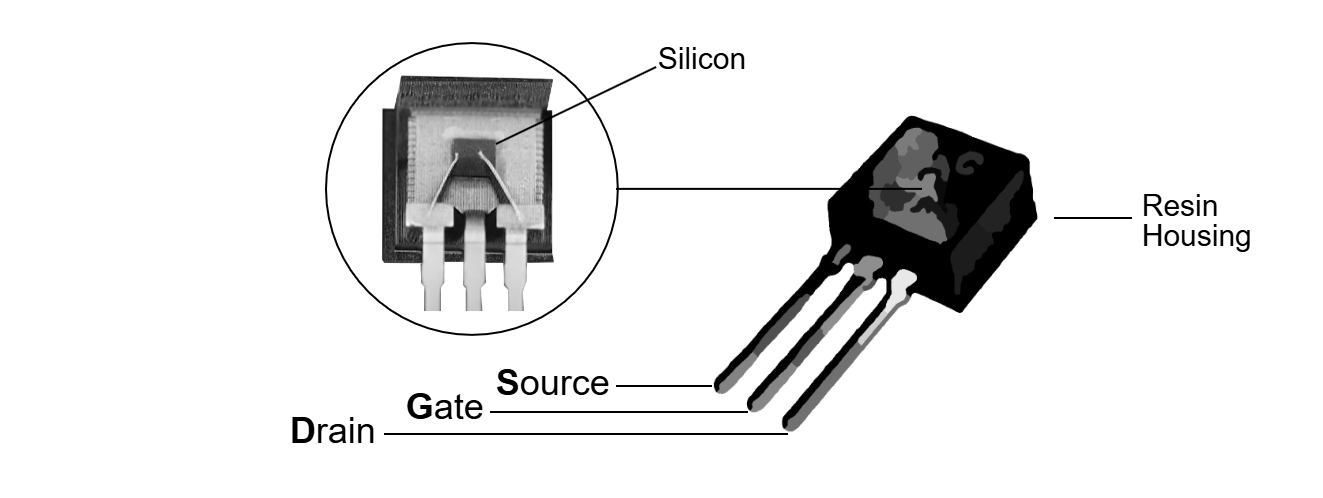
\includegraphics[width=\textwidth]{Sections/circuits/transistor.png}
  \caption{Cross-section of a discrete transistor: a silicon die (center) is bonded to three metal leads, all
    encased in an epoxy package.  A metal tab (not shown) may be added for heatsinking.}
  \label{fig:transistor}
\end{figure}

\newpage 



\begin{theo}[FETs over BJTs]

  \label{theo:why_mosfets_preferred}

  A BJT needs continuous base current, which wastes energy. A MOSFET only requires its gate to be charged or discharged (i.e., voltage applied or removed), which is more efficient.
\end{theo}

\noindent 
Now we briefly step into chemistry for completeness/review sake to understand silicon and charges:
\begin{Def}[Anotomy of an Atom]

    \label{def:atom}

    An \textbf{atom} is the smallest unit of matter that retains the properties of an element. It consists of three main subatomic particles:
    \begin{itemize}
        \item \textbf{Protons:} Positively charged particles found in the nucleus.
        \item \textbf{Neutrons:} Neutral particles also found in the nucleus (same size as protons).
        \item \textbf{Electrons:} About the same charge as proton, but negative, and about 1800x smaller and lighter than a proton.
    \end{itemize}

    \noindent
    Protons and neutrons are tightly packed together in a space called the \textbf{nucleus}, gaining the name \textbf{nucleons};
    Electrons orbit the nucleus at discrete distances called \textbf{shells} or \textbf{energy levels}. 
    \underline{The number of protons in the nucleus defines the element (i.e., specifications).} E.g., 79 protons will 
    always be gold.

    Opposite charges attract, though within an atom they never collide. Neutrons act as a buffer between protons (e.g., Silver is 
    stable with 60 or 62 neutrons, but unstable with 61). Atoms with different number of neutrons are called \textbf{isotopes}, latin for ``same place''.
    Electrons may jump between shells and atoms. If there is a greater number of electrons to protons, the atom is \textbf{negatively charged} (anions), otherwise it is \textbf{positively charged} (cations)
    \cite{crashcourse2013nucleus}.
\end{Def}

\begin{Def}[Periodic Table]

    \label{def:periodic_table}

    The \textbf{Periodic Table of Elements} organizes all known elements by the number of protons in their nuclei. This is called an \textbf{atomic number} (e.g., 
    gold's atomic number is 79). Elements are abbreviated from their latin translations (e.g., gold is \textbf{aurum}, AU, which means ``shining dawn'').
    There are 118 elements, with 80 being stable and the rest being unstable isotopes. Anything past 82 protons (lead) is 
    unstable, undergoing radioactive decay.
\end{Def}

\begin{Tip} So if you ever see a movie that says ``we discovered a new element!'' You may kindly exclaim, 
    ``That's not how it works; That's literally impossible!'' 
\end{Tip}

\newpage 

